\documentclass{article}
\usepackage[a4paper, total={6in, 8in}]{geometry}
\usepackage{graphicx}
\usepackage{url}
\usepackage{natbib}
\usepackage{todonotes}
\usepackage{booktabs}
\usepackage{lineno}
\usepackage{color}
%\usepackage{auto-pst-pdf}
\usepackage[colaction]{multicol}
\usepackage{caption}
\usepackage{svg}
\usepackage{authblk}
\usepackage{standalone}

\linespread{1.5}

\makeatletter
\renewcommand{\maketitle}{\bgroup\setlength{\parindent}{0pt}
	\begin{flushleft}

		{\huge\textbf{\@title}}

		\bigskip

 		{\large\textbf{\@author}}

 		\bigskip

 		{\large{Draft current \@date}}

	\end{flushleft}\egroup
}
\makeatother

\newcommand{\multicollinenumbers}{
	\linenumbers
	\def\makeLineNumber{\docolaction
		{\makeLineNumberLeft}
		{}
		{\makeLineNumberRight}
		}
}

\newenvironment{figurehere}
	{\def\@captype{figure}}
	{}

% Title
\title{A Topic Model of Climate Change Literature}
\title{Words, words, words: Mapping the Matter of Climate Change Literature}
\title{A Topography of Climate Change Research}
\author[1,2]{Max Callaghan}

\affil[1]{Mercator Research Institute on Global Commons and Climate Change, Torgauer Straße, 10829 Berlin, Germany}
\affil[2]{School of Earth and Environment, University of Leeds, Leeds LS2 9JT, United Kingdom}

\begin{document}
\maketitle


\begin{linenumbers}

\noindent\textbf{\documentclass{article}

\begin{document}
	The massive expansion of scientific literature on climate change poses challenges for global environmental assessments and our understanding of how these assessments work. 
	Big data and machine learning can help us deal 
	with the large collections of text represented by scientific fields.
	Such methods help make the production of assessments
	more tractable, and give us better insights about how past assessments  have engaged with the literature as it has evolved.
	We use topic modelling to identify the thematic structure and draw a comprehensive topic map, or topography, of over 400,000 scientific publications from the Web of Science (WoS) on climate change. 
	We update current knowledge on the Intergovernmental Panel on Climate Change (IPCC), showing that, at least when compared to the baseline of the literature identified in the WoS,  the social sciences are in fact over-represented in recent assessment reports, and that
	technical, solutions-relevant knowledge - especially in the agricultural and engineering sciences - are under-represented.
	We point to a variety of other applications of such maps, and our findings have direct implications for addressing growing demands for more solution-oriented climate change assessments that are also more firmly rooted in the social sciences.
	We highlight fast-growing topics on solutions that could be better integrated into future IPCC reports. 
	The perceived lack of social science knowledge in solutions-relevant IPCC reports does not necessarily imply a bias towards the natural sciences. 
	It rather suggests a need for more social science research with a focus on ``technical'' topics related to climate solutions. 
\end{document}}



\bigskip

%\begin{multicols}{2}

%\multicollinenumbers
%\bigskip
%\noindent\textbf{To deal with the wicked problem of climate change, international policy-makers need the IPCC. The IPCC as map-makers.}

The IPCC sees its role as to ``assess on a comprehensive, objective, open and transparent basis the scientific, technical and socio-economic information relevant to [...] climate change'' \citep{IPCC2013}. Climate science is so broad, multi-disciplinary, and laden with uncertainties and values, that the role of the IPCC as assessment maker is vitally important to developing evidence-based international climate policy. In the Pragmatic Enlightened Model of the science-policy interface, the task of assessment making is a cartographic one \citep{Edenhofer2015}. Assessment makers map out the problem and the option space for policy-makers.



%\bigskip
%\noindent\textbf{The task of the IPCC has become much more difficult with big literature}

Further, it has been pointed out that, in the age of ``big literature'', providing assessments that are comprehensive, objective and transparent has become much more difficult \citep{Minx2017l}. When the IPCC's citations constitute an ever-decreasing proportion of the totality of science on climate change, questions about the map that the IPCC reports produce become more pressing:

\begin{itemize}
	\item Is the map up to date?
	\item Is the map complete?
	\item Is the map's projection representative? Does it emphasise or obscure certain areas?
\end{itemize}


\section*{The IPCC as an object of scientific investigation}

%%%%%

%\bigskip
%\noindent\textbf{The IPCC, its reports and processes have been the object of study before. These are also hampered by problems of scale though}

Various researchers have attempted to do empirical research on the assessment reports, and processes of inter. alia. the IPCC \citep{jabbour2017, Bjurström2011, Corbera2016, Hulme2016}. Among the clear conclusions is that policy makers, when asked about their interactions with the IPCC call for a greater focus on solutions \citep{Kowarsch2017}. Studies that look directly at the content of IPCC reports, though, are similarly challenged by the the size of the literature that the reports assess. Without engaging with this literature, the conclusions drawn lack a reference point, and the phenomena identified (such as an over-representation of the natural sciences in IPCC citations \cite{Bjurström2011}) are hard to disentangle as specific to the way the IPCC assesses its literature, rather than a feature of the literature itself. 

%\bigskip
%\noindent\textbf{Some literature exists on bibliometrics and climate change, but tends not to deal with text}

Some studies have attempted to identify and characterise the literature on climate change through bibliometric techniques \citep{Haunschild2016, Grieneisen2011}. Such studies are the jumping off point for this work, and form the basis of the identification strategy for the literature, but they do not engage with the \textit{texts} of the work identified, nor do they make the link to the IPCC. A growing body of scientific work deals with the unsupervised analysis of texts using topic modelling \cite{Lee1999,Blei2003, Greene2016, Roberts2013}. Applications to the field of climate change though are rare and often limited to closer analysis within sub-topics \cite{Grubert2017}, or calls for their greater use \cite{Grubert2016}. 

\section*{A problem of scale}


%\bigskip
%\noindent\textbf{The scale of the problem in context}

\begin{table}
	\scriptsize
	\begin{tabular}{|l |p{1.8cm} p{1.8cm} p{1.8cm} p{1.8cm} p{1.8cm} p{1.8cm}|} 
\hline 
&\textbf{AR1} & \textbf{AR2} & \textbf{AR3} & \textbf{AR4} & \textbf{AR5} & \textbf{AR6}\\ \hline\textbf{Years} &1986-1989 & 1990-1994 & 1995-2000 & 2001-2006 & 2007-2013 & 2014-\\ 
\textbf{Documents} &1,167 & 8,539 & 21,716 & 38,750 & 134,413 & 201,606\\ 
\textbf{Unique words} &2,000 & 12,480 & 23,346 & 34,637 & 71,867 & 94,746\\ 
\textbf{New words} & change (560) & oil (287) & downscaling (217) & sres (234) & biochar (1,791) & mmms (313)\\ & climate (428) & deltac (283) & degreesc (187) & petm (95) & redd (1,113) & cop21 (234)\\ & co2 (318) & whole (256) & ncep (130) & amf (88) & cmip5 (679) & c3n4 (214)\\ & climatic (289) & tax (254) & fco (107) & sf5cf3 (86) & cmip3 (587) & sdg (187)\\ & model (288) & landscape (249) & pfc (98) & clc (81) & mofs (299) & zika (182)\\ & atmospheric (281) & alternative (243) & otcs (98) & embankment (81) & sdm (297) & ndcs (168)\\ & effect (280) & availability (242) & dtr (95) & cwd (79) & mof (275) & indc (164)\\ & global (224) & life (239) & nee (89) & etm (75) & biochars (252) & indcs (134) \\ \hline
\end{tabular}

	\caption{Growth in climate change literature}
	\label{growthtable}
\end{table}

The case for a greater application of text-mining approaches in understanding and assisting the IPCC is made by the scale of the challenge it faces, depicted in table \ref{growthtable}. Less than a thousand documents relevant to climate change were published before the first assessment report (see Methods for data, exclusions and processing). The abstracts of these documents contained 1,380 unique terms. In the three complete years since the publication of AR5, 128,266 documents have been published, containing 74,196 unique terms. The new words in each assessment period unearthed by a basic machine-reading of the literature already give an indication of the how the field has expanded. They chart the emergence of

\linespread{1}
\begin{itemize}
	\item new compounds or materials, such as trifluoromethyl sulfur pentafluoride (SF5CF3) in AR4, or mixed matrix membranes (MMMs) in AR6
	\item new models, or modelling approaches, such as HadCM2 in AR3, or CMIP in AR5 and AR6.
	\item the involvement of new actors, such as NCEP (National Centers for Environmental Prediction) in AR3
	\item new approaches, such as biochar and REDD in AR5
	\item new applications of equipment, such as OTCs (Open-top Chambers) in AR3;
	\item new phenomena in relation to climate change, such as zika and twitter;
	\item and new concepts, such as CO2 fugacity (fco) in AR3
\end{itemize}
\linespread{1.5}




%To put this into context, the 1,189 chapters of the Bible contain a vocabulary of 11,977 unique words. Put another way, 
To put this growth into context, the 236,634 publications published in AR5 and AR6 are significantly larger than the 178,118 publications recorded in the first volume of the `Catalogue of Scientific Papers', compiled by the Royal Society to record the entirety of scientific output from 1800 to 1863 \citep{Csiszar2017}. In the last 10 years, climate science has produced significantly more papers than the were published across all scientific disciplines in the first half of the 19th Century.




%\begin{figure}
%	\begin{center}
%		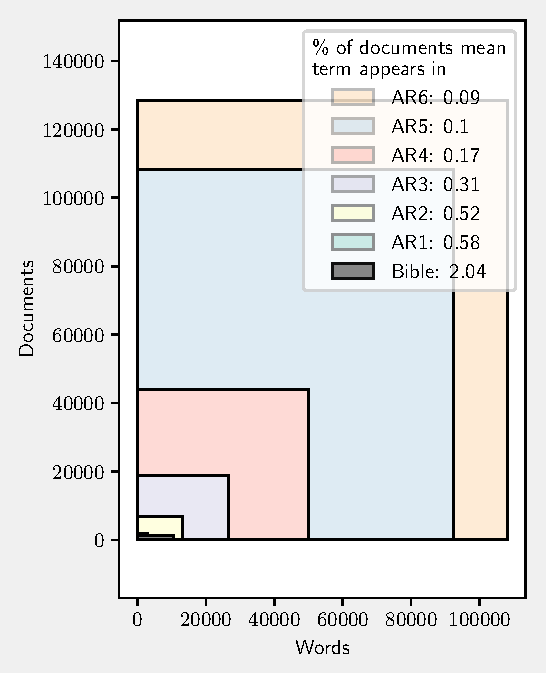
\includegraphics[width=0.5\linewidth]{plots/literature_size/volume_variety.pdf}
%		%\captionof{figure}
%		\caption{The volume and variety of literature on climate change has grown to unmanageable proportions. Each box represents a document-term matrix (unique documents x unique terms) of the abstracts written in each assessment period. The percentage of documents in which the average word occurs in is given in the key.
%		}
%		\label{growth}
%	\end{center}
%\end{figure}


%\bigskip
%\noindent\textbf{Machine reading to deal with scale problems in the making and assessing of maps}


Clearly, if the IPCC is to continue producing comprehensive assessments, it has to engage in machine-reading in order to remain anchored to the wider literature. Without such an approach, it becomes harder to justify which ever-diminishing proportion of the wider literature is included in assessments. The same arguement holds for scholars and critics of the IPCC. Without machine reading the literature at large, it becomes harder to analyse or criticise, with quantitatively evidenced claims, the outcomes of assessment processes.


%\bigskip
%\noindent\textbf{Dimension reduction makes possible the description in reduced form, and with less human bias, of unmanageably large datasets}

%\citep{Greene2016} \citep{Lee1999}
In order to draw substantive messages from this high-dimensional document-word space, we apply a form of dimensionality reduction called topic-modelling \citep{Blei2010}. The non-negative matrix factorisation (NMF) approach to topic modelling is based on generating a ``perception of the whole based on perception of its parts'' \citep{Lee1999}. Here the corpus of documents (whole) is summarised by its parts (topics), which appear in varying proportions in each of the documents. Importantly, in such approaches, the parts are not pre-defined, but learned by the algorithm, leveraging systematic co-occurences of words within documents. This makes the discovery of unlooked-for features possible and can reduce the human bias risked by the pre-definition of categories. 

%\bigskip
%\noindent\textbf{Machine reading is a supplement to assessment-making and not free from bias; a topography is not a map}

Despite these advantages, machine reading and machine learning approaches can of course not replace the task of human assessment-making. The contribution that could be made, though, is to pre-process the literature, producing a topographical map, used to navigate the literature while producing a more detailed assessment with human judgement. In fact this happens already - when IPCC authors search for literature on a topic, the results which appear on the search engine they use will be subject to algorithms based on the processing of millions of records of article text and metadata. This can be done in a much more systematic way when scientists perform directed analyses of the literature at scale. 


%\bigskip
%\noindent\textbf{This study's contribution. Overarching themes, structure of the literature, development, relation to IPCC}

In applying a dynamic version of NMF \cite{Greene2016}, this study demonstrates how topic modelling can be used to gain an overview of an otherwise unmanageably large body of literature. This overview, or topography, describes the thematic development of the climate change literature and, in a novelly systematic way, examines how comprehensively the IPCC has been able to engage with it. In pulling together strands from text-mining, bibliometrics, and the study of science and policy, this study advances our understanding of the literature on climate change and the role of the IPCC in communicating this to policy makers.


\section*{Results}

Table \ref{top-topics} shows the 10 most prominent topics within the literature on climate change. The topics are characterised by the (stemmed) words that define them, and by the documents which are most well described by them. For example, the topic ``energi, renew, consumpt'' features the words energi, renew, consumpt,
effici, demand,
save, sector, sourc,
industri, use, and best describes the documents ``Energy issues and energy priorities'' \cite{Demirbas2008} and ``Energy efficiency and CO2 emissions in Swedish manufacturing industries'' \cite{PardoMartinez2013}. The topics learned by dynamic NMF identify a set of interpretable topics and can identify which documents belong to these topics. 

\begin{table}
	\scriptsize
	\begin{tabular}{p{1.9cm} p{3cm} p{7.5cm} r}
\toprule
                      title &                                                                            top words &                                                                                                                                                                                                                                                                top docs &   share \\
\midrule
      climat, chang, impact &          [climat, chang, impact, respons, futur, effect, shift, sensit, affect, may] &                                                                                                                                                  \parbox[t]{7.5cm}{Climate oscillations and changes over Russia; \\World Regionalization of Climate Change (1961-2010)} &  2.73\% \\
     soil, moistur, microbi &       [soil, moistur, microbi, organ, respir, content, miner, depth, matter, efflux] &                                                                                    \parbox[t]{7.5cm}{PARTITIONING OF SOIL RESPIRATION IN A FIRST ROTATION BEECH PLANTATION; \\Responses of soil respiration to N fertilization in a loamy soil under maize cultivation} &  2.73\% \\
       emiss, reduct, reduc &      [emiss, reduct, reduc, greenhous, factor, total, estim, inventori, nox, measur] &                                                                                                             \parbox[t]{7.5cm}{China's CH4 and CO2 emissions: Bottom-up estimation and comparative analysis; \\Monitoring total emissions from industrial installations} &  2.21\% \\
   carbon, dioxid, sequestr &   [carbon, dioxid, sequestr, sink, organ, cycl, storag, stock, terrestri, atmospher] &                             \parbox[t]{7.5cm}{Interpreting carbon-isotope excursions: carbonates and organic matter; \\PARTICULATE FLUXES OF CARBONATE AND ORGANIC-CARBON IN THE OCEAN - IS THE MARINE BIOLOGICAL-ACTIVITY WORKING AS A SINK OF THE ATMOSPHERIC CARBON} &  1.74\% \\
      temperatur, air, mean &  [temperatur, air, mean, surfac, minimum, maximum, daili, increas, effect, degreesc] &                                                                                                     \parbox[t]{7.5cm}{Observed changes in shallow soil temperatures in Northeast China, 1960-2007; \\Beyond the Mean: Biological Impacts of Cryptic Temperature Change} &  1.71\% \\
      record, dure, glacial &       [record, dure, glacial, reconstruct, last, period, holocen, event, late, core] &                                                           \parbox[t]{7.5cm}{HIGH-RESOLUTION CLIMATE RECORDS FROM THE NORTH-ATLANTIC DURING THE LAST INTERGLACIAL; \\HIGH-RESOLUTION CLIMATIC INFORMATION FROM SHORT FIRN CORES, WESTERN DRONNING MAUD LAND, ANTARCTICA} &   1.7\% \\
     speci, distribut, rang &          [speci, distribut, rang, rich, invas, nich, predict, extinct, shift, abund] &                               \parbox[t]{7.5cm}{Northward range extensions of some mesopelagic fishes in the Northeastern Atlantic; \\Natural occurrence and backwater infection of C-4 plants in the vegetation of the Yangtze hydropower Three Gorges Project region} &   1.7\% \\
 increas, concentr, decreas &   [increas, concentr, decreas, effect, atmospher, doc, result, organ, nutrient, may] &                                                          \parbox[t]{7.5cm}{TERRESTRIAL HIGHER-PLANT RESPONSE TO INCREASING ATMOSPHERIC [CO2] IN RELATION TO THE GLOBAL CARBON-CYCLE; \\Hydrological response to climate change in the Black Hills of South Dakota, USA} &  1.61\% \\
      forest, tropic, stand &       [forest, tropic, stand, deforest, disturb, stock, boreal, redd, harvest, wood] &  \parbox[t]{7.5cm}{Spatially explicit estimates and temporal changes of forest tree biomass in a typical department of forest management, Turkey; \\Analysis of the changes in forest ecosystem functions, structure and composition in the Black Sea region of Turkey} &  1.56\% \\
    energi, renew, consumpt &        [energi, renew, consumpt, effici, demand, save, sector, sourc, industri, use] &                                                                                                                                       \parbox[t]{7.5cm}{Energy issues and energy priorities; \\Energy efficiency and CO2 emissions in Swedish manufacturing industries} &  1.56\% \\
\bottomrule
\end{tabular}

	\caption{Top 10 topics in climate change literature}
	\label{top-topics}
\end{table}

Such first results show the promise of topic modelling in the identification of studies in a thematic area, which is of high value to assessment exercises like the IPCC, but in themselves do not give a sense of the broad structure of the corpus. Figure \ref{map-double} projects the documents on to a two dimensional representation of the their topic composition derived through t-distributed Stochastic Network Embedding (t-SNE) \cite{vandermaaten2008}. In this approach, documents are positioned close to other documents with similar topic compositions. This projection enables us to show a topography of the whole literature on climate change.

\begin{figure}
	\begin{center}
		%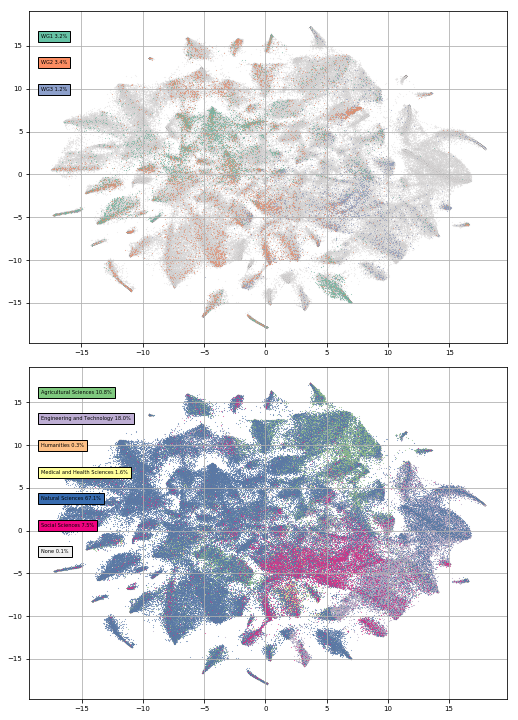
\includegraphics[width=1\linewidth]{tsne_results/plots/run_665_s_0_p200_double.pdf}
		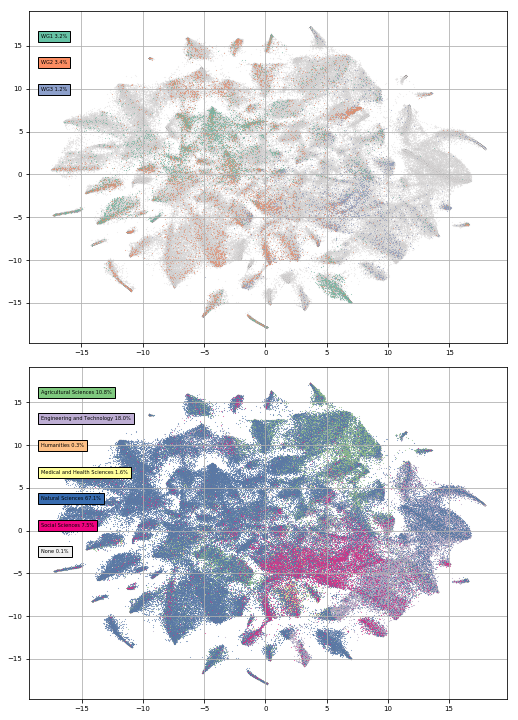
\includegraphics[width=0.85\linewidth]{tsne_results/plots/run_665_s_0_p200_double.png}
		\caption{A map of the literature on climate change. Document positions are obtained by reducing the topic scores to two dimensions via t-SNE Documents are coloured by working group citations (top) and web of science discipline category (bottom). See SI table for topic composition of each grid square}
		\label{map-double}
	\end{center}
\end{figure}


In the two panels of the figure, the documents are coloured by the IPCC working group which cites them (if any), and the disciplinary classification according to the Web of Science. The topic structure cuts across working group and disciplinary lines, but the disciplinary and working group structure is clearly visible in the topography. For example, in the south-eastern section of the map, we can see a concentration of documents in the social sciences that were cited by working group III (mitigation).

The topography\_map\_reference.csv file in the supporting materials aids more detailed analysis of the map, describing the topic composition of each square. For example the square whose center is [12.5,-7.5] is made up of the topics \{energi, renew, consumpt\}, \{fuel, fossil, engin\}, \{emiss, reduct, reduc\}, \{countri, develop, trade\} and \{cost, optim, price\}, typical social science, working group III topics. The square whose center is [-17.5,-2.5], containing mostly working group I documents on the other hand, is made of largely by the topic {ozon, stratospher, tropospher} as well as by {increas, concentr, decreas}, and {climat, chang, impact}.

%\bigskip
%\noindent\textbf{A topographical map of climate change documents shows the broad structure of climate change literature}


\begin{figure}
	\begin{center}
		%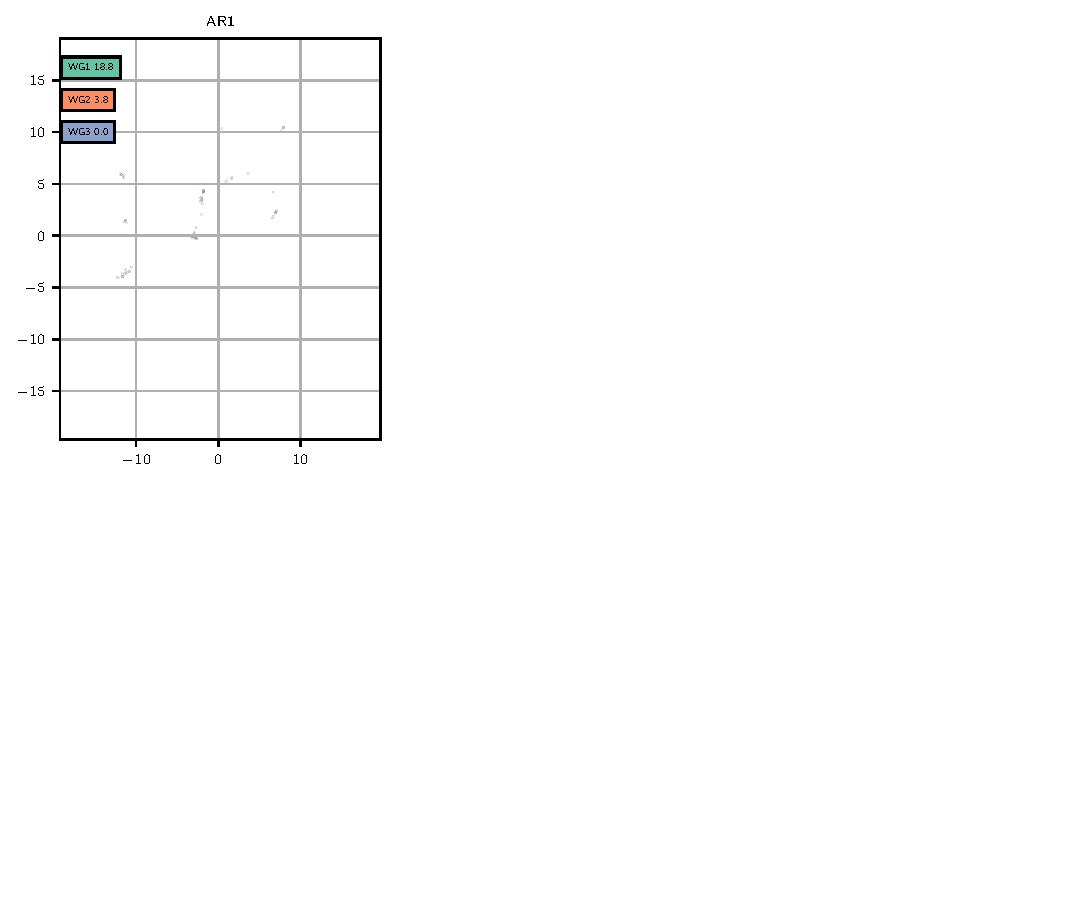
\includegraphics[width=1\linewidth]{tsne_results/plots/run_665_s_0_p200_evolution.pdf}
		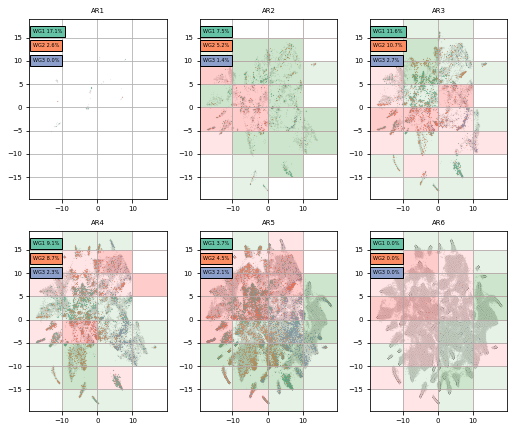
\includegraphics[width=1\linewidth]{tsne_results/plots/run_665_s_0_p200_evolution.png}
		\caption{The evolution of the landscape of climate change literature}
		\label{}
	\end{center}
\end{figure}


%\begin{figure}
%	\begin{center}
%		%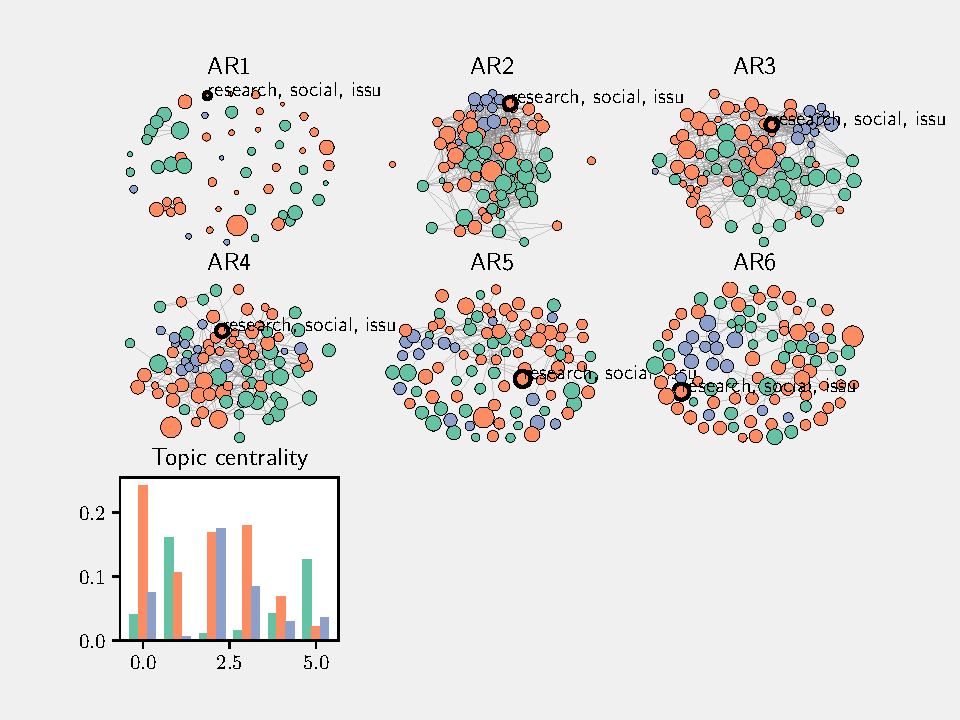
\includegraphics[width=1\linewidth]{plots/network_development_wgs_665.pdf}
%		\caption{The development of the topic-document correlation network over IPCC assessment periods.}
%		\label{}
%	\end{center}
%\end{figure}

%\bigskip
%\noindent\textbf{The topic-document correlation network is densest in AR2 and 3 but becomes more fragmented over time}
%
%(partly: Model less good at describing literature later on)

%\bigskip
%\noindent\textbf{Working groups are clustered together [dynamics], with topics like [x] containing documents across working groups and topics like [y] important network nodes}


\begin{figure}
	\begin{center}
		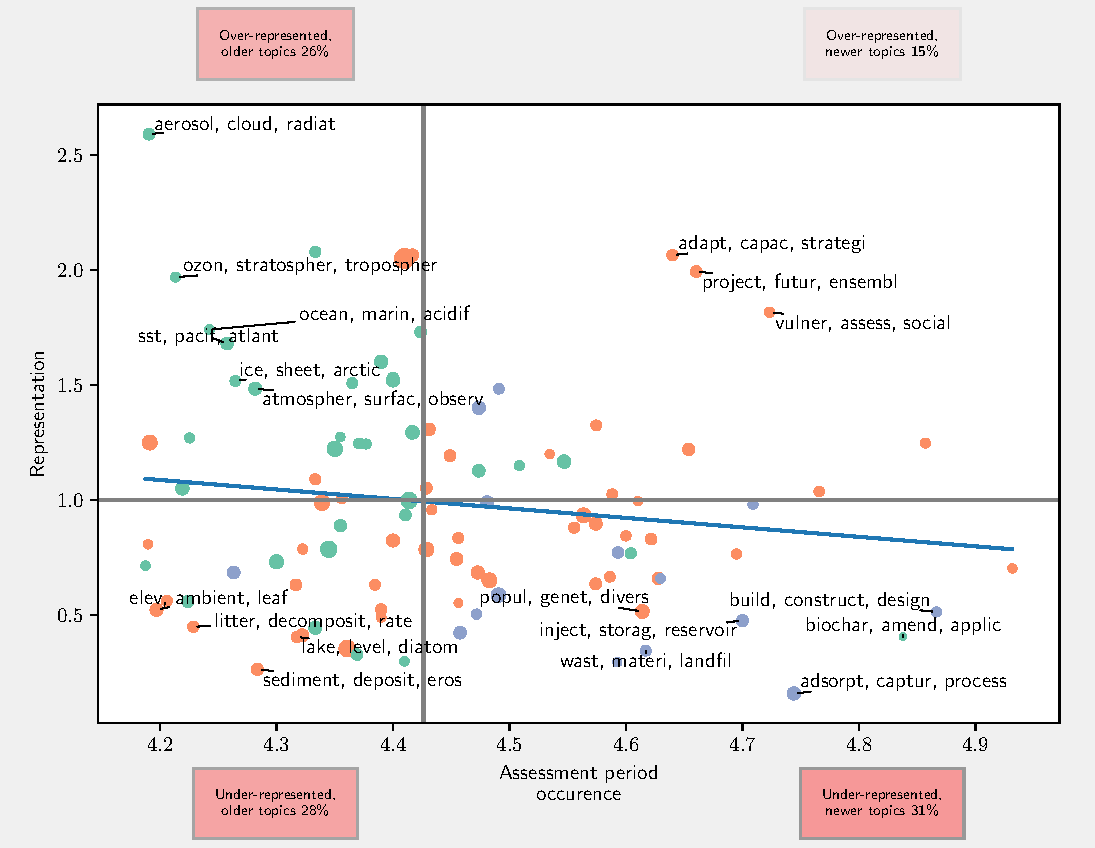
\includegraphics[width=1\linewidth]{plots/ipcc_representation/ipcc_rep_new665_all.pdf}
		\caption{Representation and newness of dynamic topics}
		\label{}
	\end{center}
\end{figure}


\bigskip
\noindent\textbf{Sustainability has been an increasingly important theme in an overarching topic about environmental sciences}

(compare to biochar, which is much more recent)

\begin{figure}
	\begin{center}
		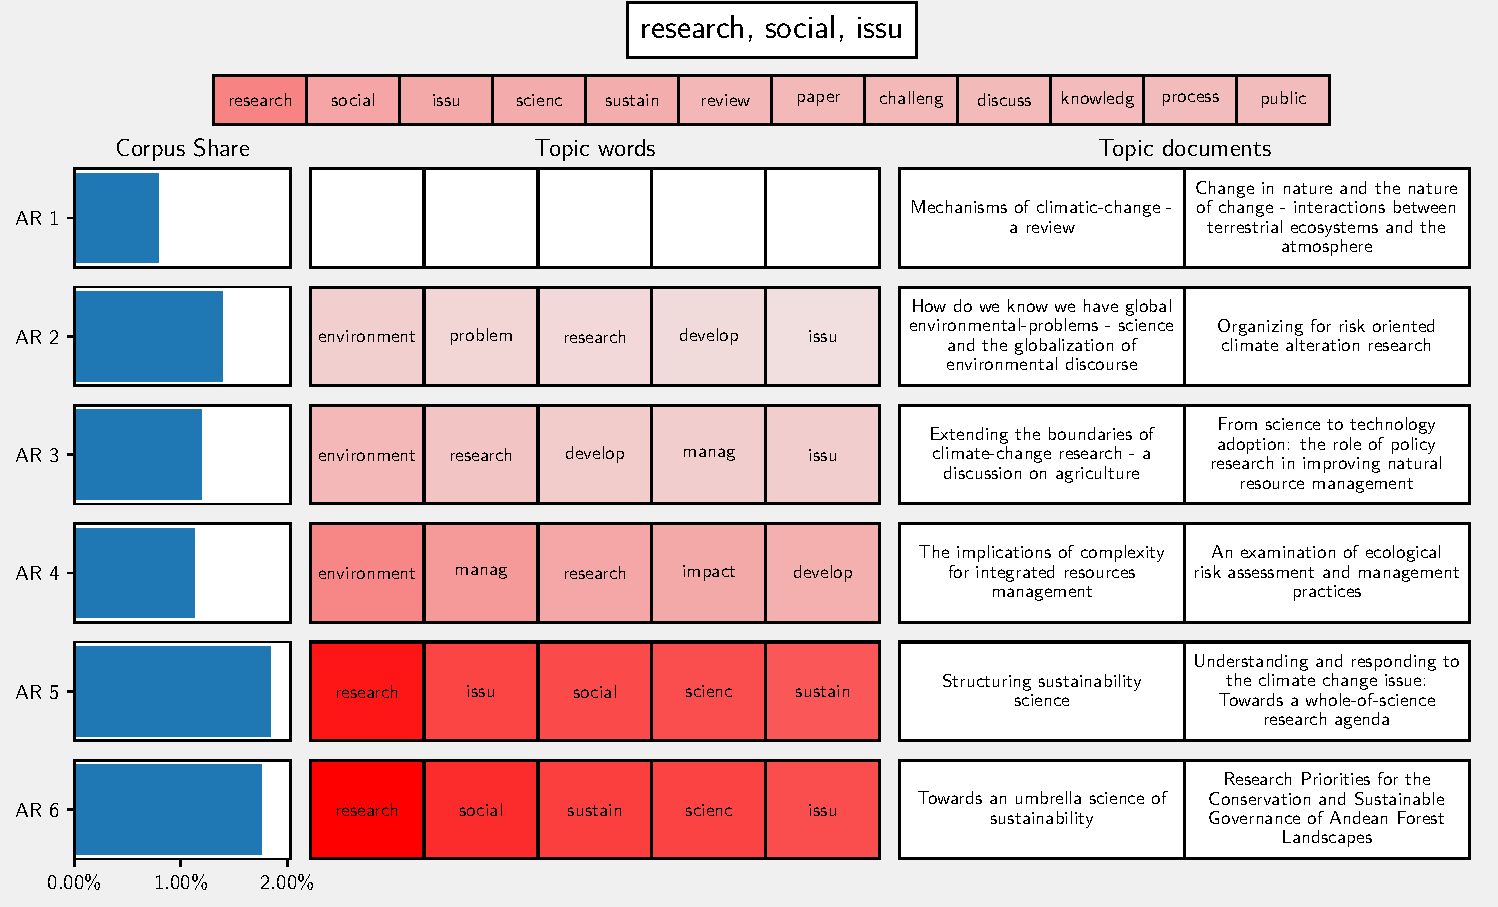
\includegraphics[width=1\linewidth]{plots/single_topic_3_11046.pdf}
		\caption{Word and document development of the ``Research'' dynamic topic}
		\label{}
	\end{center}
\end{figure}

\begin{figure}
	\begin{center}
		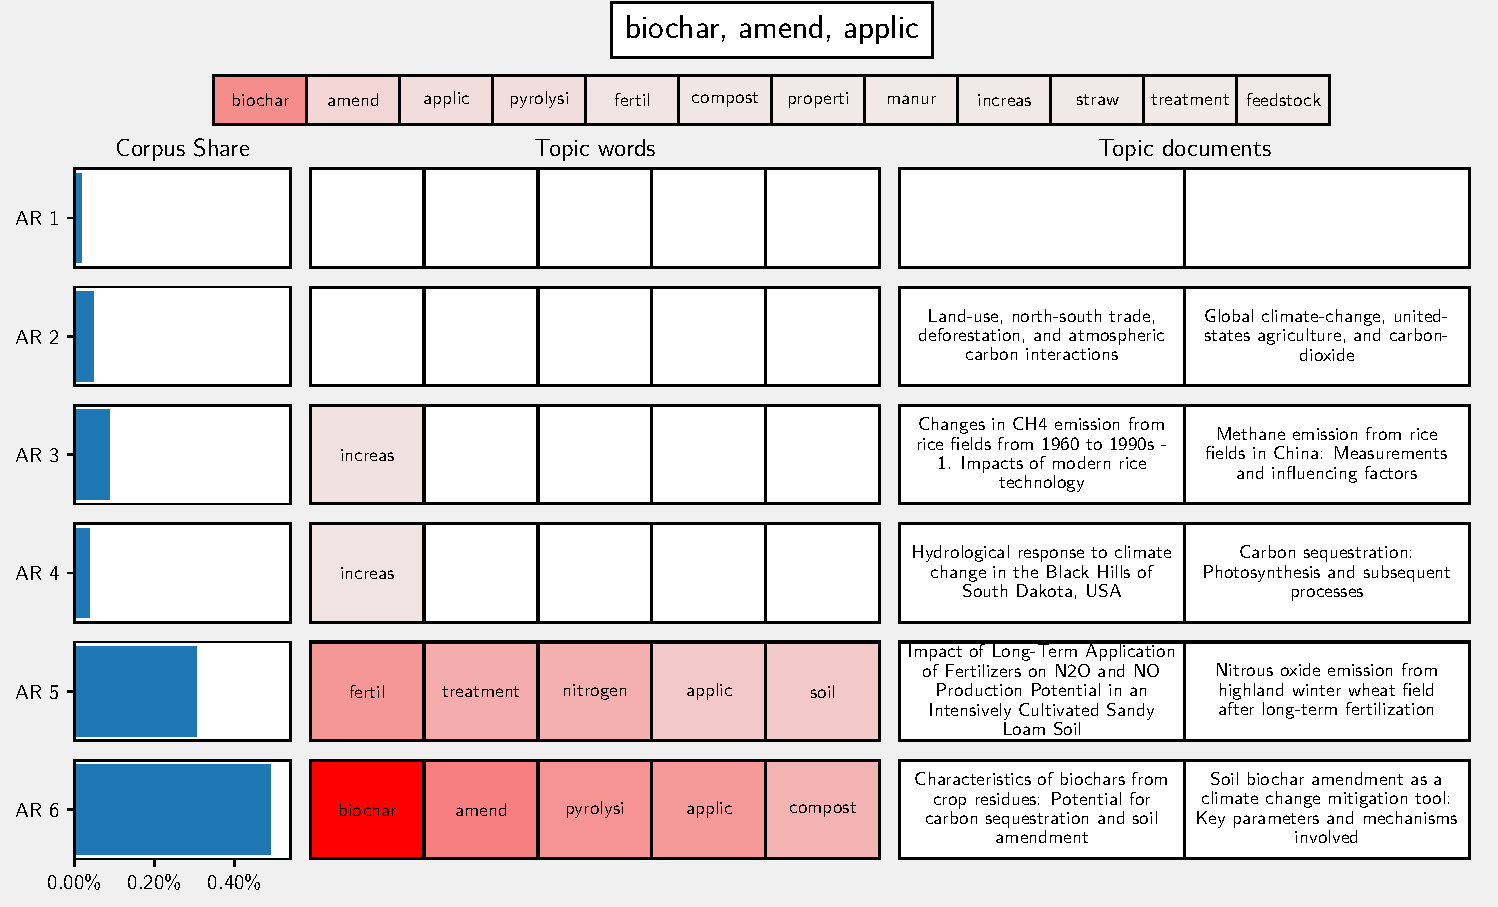
\includegraphics[width=1\linewidth]{plots/single_topic_3_11020.pdf}
		\caption{SI Word and document development of the ``Biochar'' dynamic topic}
		\label{}
	\end{center}
\end{figure}


\begin{figure}
\begin{center}
	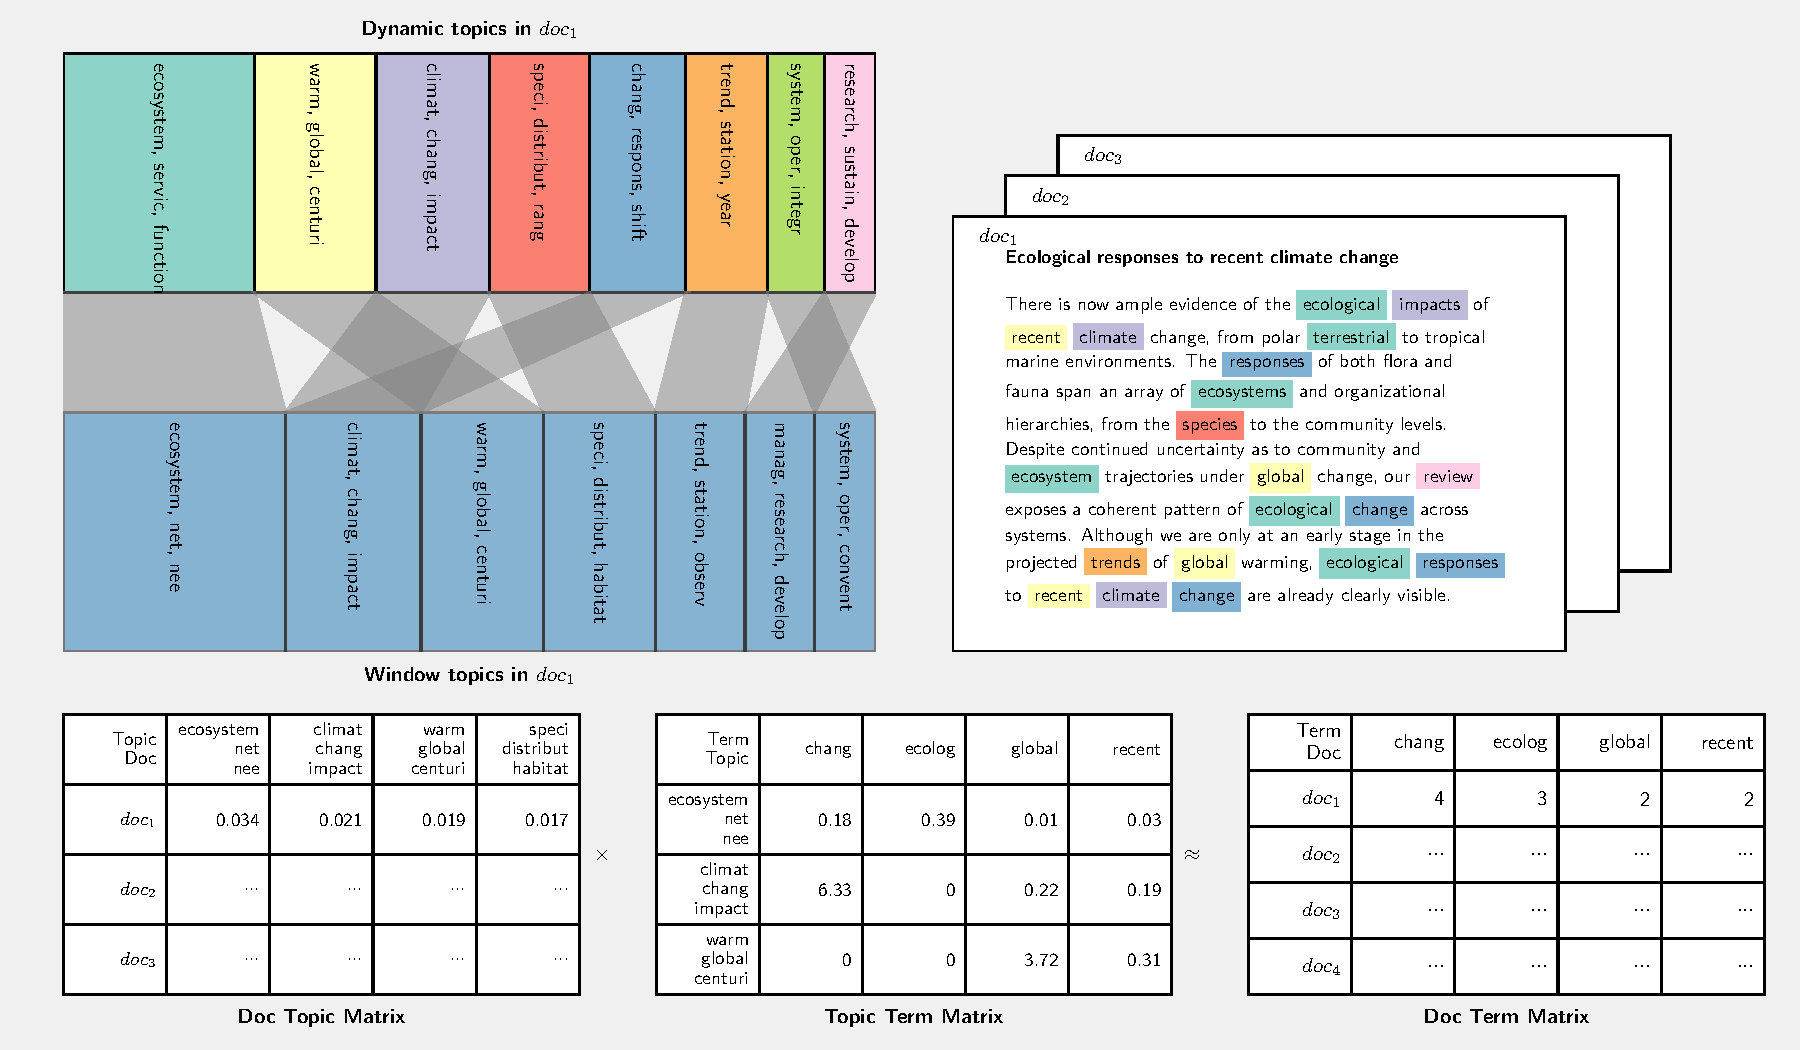
\includegraphics[width=1\linewidth]{plots/single_doc_3_536594.pdf}
    \caption{SI Topic make up of a single document}
    \label{}
    \end{center}
\end{figure}

\bigskip
\noindent\textbf{Physical science topics tend to be the oldest, and the most well represented topics}

\bigskip
\noindent\textbf{Adaptation and impact studies have seen a lot of growth but are well represented in IPCC reports}

\bigskip
\noindent\textbf{New topics around negative emissions and urban form are very recent and not well represented in IPCC reports.}

Negative emissions in special report on 1.5, demand side chapter in AR6



\section*{Discussion}

\bigskip
\noindent\textbf{Solutions, policies and science}

What do policy-makers mean when they ask for more solutions

\bigskip
\noindent\textbf{Perfect representation is not necessarily desirable, but the skewedness should be known}

There may be good reasons for a topic to be less prominent in IPCC discussions than in the wider scientific literature, and these reasons can only be understood and acted upon by humans, not by machine-reading. Nevertheless, it is desirable that assessment makers are aware of the relationship

%Increase in the frequency of the use of the term ``solutions'' \citep{jabbour2017},

\section*{Methods}
\label{methods}



\subsection*{Data}
%This study reproduces the query developed by \citep{Grieneisen2011}, which is carried out on Web of Science. Though not exhaustive, it gives a good coverage of

\end{linenumbers}

%\end{multicols}

%\listoffigures
%\linespread{1}
%\bibliography{Mendeley}
%\bibliographystyle{unsrt}

\end{document}
